% Options for packages loaded elsewhere
\PassOptionsToPackage{unicode}{hyperref}
\PassOptionsToPackage{hyphens}{url}
%
\documentclass[
]{book}
\usepackage{amsmath,amssymb}
\usepackage{iftex}
\ifPDFTeX
  \usepackage[T1]{fontenc}
  \usepackage[utf8]{inputenc}
  \usepackage{textcomp} % provide euro and other symbols
\else % if luatex or xetex
  \usepackage{unicode-math} % this also loads fontspec
  \defaultfontfeatures{Scale=MatchLowercase}
  \defaultfontfeatures[\rmfamily]{Ligatures=TeX,Scale=1}
\fi
\usepackage{lmodern}
\ifPDFTeX\else
  % xetex/luatex font selection
\fi
% Use upquote if available, for straight quotes in verbatim environments
\IfFileExists{upquote.sty}{\usepackage{upquote}}{}
\IfFileExists{microtype.sty}{% use microtype if available
  \usepackage[]{microtype}
  \UseMicrotypeSet[protrusion]{basicmath} % disable protrusion for tt fonts
}{}
\makeatletter
\@ifundefined{KOMAClassName}{% if non-KOMA class
  \IfFileExists{parskip.sty}{%
    \usepackage{parskip}
  }{% else
    \setlength{\parindent}{0pt}
    \setlength{\parskip}{6pt plus 2pt minus 1pt}}
}{% if KOMA class
  \KOMAoptions{parskip=half}}
\makeatother
\usepackage{xcolor}
\usepackage{color}
\usepackage{fancyvrb}
\newcommand{\VerbBar}{|}
\newcommand{\VERB}{\Verb[commandchars=\\\{\}]}
\DefineVerbatimEnvironment{Highlighting}{Verbatim}{commandchars=\\\{\}}
% Add ',fontsize=\small' for more characters per line
\usepackage{framed}
\definecolor{shadecolor}{RGB}{248,248,248}
\newenvironment{Shaded}{\begin{snugshade}}{\end{snugshade}}
\newcommand{\AlertTok}[1]{\textcolor[rgb]{0.94,0.16,0.16}{#1}}
\newcommand{\AnnotationTok}[1]{\textcolor[rgb]{0.56,0.35,0.01}{\textbf{\textit{#1}}}}
\newcommand{\AttributeTok}[1]{\textcolor[rgb]{0.13,0.29,0.53}{#1}}
\newcommand{\BaseNTok}[1]{\textcolor[rgb]{0.00,0.00,0.81}{#1}}
\newcommand{\BuiltInTok}[1]{#1}
\newcommand{\CharTok}[1]{\textcolor[rgb]{0.31,0.60,0.02}{#1}}
\newcommand{\CommentTok}[1]{\textcolor[rgb]{0.56,0.35,0.01}{\textit{#1}}}
\newcommand{\CommentVarTok}[1]{\textcolor[rgb]{0.56,0.35,0.01}{\textbf{\textit{#1}}}}
\newcommand{\ConstantTok}[1]{\textcolor[rgb]{0.56,0.35,0.01}{#1}}
\newcommand{\ControlFlowTok}[1]{\textcolor[rgb]{0.13,0.29,0.53}{\textbf{#1}}}
\newcommand{\DataTypeTok}[1]{\textcolor[rgb]{0.13,0.29,0.53}{#1}}
\newcommand{\DecValTok}[1]{\textcolor[rgb]{0.00,0.00,0.81}{#1}}
\newcommand{\DocumentationTok}[1]{\textcolor[rgb]{0.56,0.35,0.01}{\textbf{\textit{#1}}}}
\newcommand{\ErrorTok}[1]{\textcolor[rgb]{0.64,0.00,0.00}{\textbf{#1}}}
\newcommand{\ExtensionTok}[1]{#1}
\newcommand{\FloatTok}[1]{\textcolor[rgb]{0.00,0.00,0.81}{#1}}
\newcommand{\FunctionTok}[1]{\textcolor[rgb]{0.13,0.29,0.53}{\textbf{#1}}}
\newcommand{\ImportTok}[1]{#1}
\newcommand{\InformationTok}[1]{\textcolor[rgb]{0.56,0.35,0.01}{\textbf{\textit{#1}}}}
\newcommand{\KeywordTok}[1]{\textcolor[rgb]{0.13,0.29,0.53}{\textbf{#1}}}
\newcommand{\NormalTok}[1]{#1}
\newcommand{\OperatorTok}[1]{\textcolor[rgb]{0.81,0.36,0.00}{\textbf{#1}}}
\newcommand{\OtherTok}[1]{\textcolor[rgb]{0.56,0.35,0.01}{#1}}
\newcommand{\PreprocessorTok}[1]{\textcolor[rgb]{0.56,0.35,0.01}{\textit{#1}}}
\newcommand{\RegionMarkerTok}[1]{#1}
\newcommand{\SpecialCharTok}[1]{\textcolor[rgb]{0.81,0.36,0.00}{\textbf{#1}}}
\newcommand{\SpecialStringTok}[1]{\textcolor[rgb]{0.31,0.60,0.02}{#1}}
\newcommand{\StringTok}[1]{\textcolor[rgb]{0.31,0.60,0.02}{#1}}
\newcommand{\VariableTok}[1]{\textcolor[rgb]{0.00,0.00,0.00}{#1}}
\newcommand{\VerbatimStringTok}[1]{\textcolor[rgb]{0.31,0.60,0.02}{#1}}
\newcommand{\WarningTok}[1]{\textcolor[rgb]{0.56,0.35,0.01}{\textbf{\textit{#1}}}}
\usepackage{longtable,booktabs,array}
\usepackage{calc} % for calculating minipage widths
% Correct order of tables after \paragraph or \subparagraph
\usepackage{etoolbox}
\makeatletter
\patchcmd\longtable{\par}{\if@noskipsec\mbox{}\fi\par}{}{}
\makeatother
% Allow footnotes in longtable head/foot
\IfFileExists{footnotehyper.sty}{\usepackage{footnotehyper}}{\usepackage{footnote}}
\makesavenoteenv{longtable}
\usepackage{graphicx}
\makeatletter
\def\maxwidth{\ifdim\Gin@nat@width>\linewidth\linewidth\else\Gin@nat@width\fi}
\def\maxheight{\ifdim\Gin@nat@height>\textheight\textheight\else\Gin@nat@height\fi}
\makeatother
% Scale images if necessary, so that they will not overflow the page
% margins by default, and it is still possible to overwrite the defaults
% using explicit options in \includegraphics[width, height, ...]{}
\setkeys{Gin}{width=\maxwidth,height=\maxheight,keepaspectratio}
% Set default figure placement to htbp
\makeatletter
\def\fps@figure{htbp}
\makeatother
\setlength{\emergencystretch}{3em} % prevent overfull lines
\providecommand{\tightlist}{%
  \setlength{\itemsep}{0pt}\setlength{\parskip}{0pt}}
\setcounter{secnumdepth}{5}
\usepackage{booktabs}
\ifLuaTeX
  \usepackage{selnolig}  % disable illegal ligatures
\fi
\usepackage[]{natbib}
\bibliographystyle{plainnat}
\IfFileExists{bookmark.sty}{\usepackage{bookmark}}{\usepackage{hyperref}}
\IfFileExists{xurl.sty}{\usepackage{xurl}}{} % add URL line breaks if available
\urlstyle{same}
\hypersetup{
  pdftitle={CC Primer: Compute Canada for geoscientists in a rush},
  pdfauthor={Ricardo Barros Lourenco},
  hidelinks,
  pdfcreator={LaTeX via pandoc}}

\title{CC Primer: Compute Canada for geoscientists in a rush}
\author{Ricardo Barros Lourenco}
\date{Last revision: 2023-10-13}

\begin{document}
\maketitle

{
\setcounter{tocdepth}{1}
\tableofcontents
}
\hypertarget{front-matter}{%
\chapter{Front Matter}\label{front-matter}}

\hypertarget{copyright}{%
\section{Copyright}\label{copyright}}

Otherwise stated in the text, this content is licensed under a \href{http://creativecommons.org/licenses/by-nc-sa/4.0/}{Creative Commons Attribution-NonCommercial-ShareAlike 4.0 International License}.

\hypertarget{how-to-cite-this-work}{%
\subsection{How to cite this work}\label{how-to-cite-this-work}}

Please use this BibTeX fragment:

\begin{Shaded}
\begin{Highlighting}[]
\SpecialCharTok{@}\NormalTok{book\{BarrosLourenco2022,}
\NormalTok{  title     }\OtherTok{=} \StringTok{"CC Primer: Compute Canada for geoscientists in a rush"}\NormalTok{,}
\NormalTok{  author    }\OtherTok{=} \StringTok{"Barros Lourenco, Ricardo"}\NormalTok{,}
\NormalTok{  year      }\OtherTok{=} \DecValTok{2022}\NormalTok{,}
\NormalTok{  doi       }\OtherTok{=} \StringTok{"10.5281/zenodo.5937906"}
\NormalTok{  note      }\OtherTok{=}\NormalTok{ \{\textbackslash{}url\{https}\SpecialCharTok{:}\ErrorTok{//}\NormalTok{ricardobarroslourenco.github.io}\SpecialCharTok{/}\NormalTok{CCprimer}\SpecialCharTok{/}\NormalTok{\}(visited yyyy}\SpecialCharTok{{-}}\NormalTok{mm}\SpecialCharTok{{-}}\NormalTok{dd)\}}
\NormalTok{\}}
\end{Highlighting}
\end{Shaded}

Obs.: Note that the DOI is of the base version (10.5281/zenodo.5937906) when
compared to each revision releases, because it relates to all versions
of this document, rather than a especific one.

\hypertarget{dedication}{%
\section{Dedication}\label{dedication}}

The author dedicates this work to all geoscientists that are trying to cross the
border into Computational Sciences, and to all computer scientists, mathematicians,
physicists, and other professionals who daily contribute in this community,
by writing code, documenting, answering questions, maintaining infrastructure,
among many other essential tasks. Thank you for your service!

\hypertarget{epigraph}{%
\section{Epigraph}\label{epigraph}}

\begin{quote}
``Here's to the crazy ones.
The misfits.
The rebels.
The troublemakers.
The round pegs in the square holes.

The ones who see things differently.

They're not fond of rules.
And they have no respect for the status quo.

You can quote them, disagree with them, glorify or vilify them.
About the only thing you can't do is ignore them.

Because they change things.

They push the human race forward.

While some may see them as the crazy ones,
we see genius.

Because the people who are crazy enough to think
they can change the world, are the ones who do.''

--- Apple Computer, \emph{``Think different''} campaign. TBWA-Chiat-Day.
\end{quote}

\hypertarget{acknowledgements}{%
\section{Acknowledgements}\label{acknowledgements}}

The author would like to acknowledge the contibution of the general Open Source Science
community, in especially the following entities:

\begin{itemize}
\tightlist
\item
  \href{https://www.anaconda.com/}{Anaconda}
\item
  \href{https://alliancecan.ca/}{Digital Research Alliance of Canada} (formerly Compute Canada)
\item
  \href{https://www.globus.org}{Globus}
\item
  \href{https://pangeo.io}{Pangeo Community}
\item
  \href{https://rocker-project.org}{RockeR Project}
\item
  \href{https://scholar.google.com/citations?user=RTF50S4AAAAJ}{Vanessa Sochat}
\end{itemize}

The author would like to acknowledge support, in part, of the following on this
work:

\begin{itemize}
\tightlist
\item
  Through my advisor, Prof.~\href{https://scholar.google.ca/citations?user=snRPOMkAAAAJ}{Alemu Gonsamo}:

  \begin{itemize}
  \tightlist
  \item
    Natural Sciences and Engineering Research Council of Canada (NSERC), through its NSERC
    Alliance program (Application: ALLRP 566310-21)
  \item
    Canada Research Chair program (CRC-2019-00139)
  \end{itemize}
\item
  \href{https://climate.mcmaster.ca}{McMaster University Centre for Climate Change} Research Seed Fund
\item
  The Shared Hierarchical Academic Research Computing Network (\href{https://www.sharcnet.ca/}{SHARCNET}), and
  the Digital Research Alliance of Canada through its Research Allocation Competition, under the
  2023 Resources for Research Groups process ``National carbon flux estimation system for forest
  ecosystems of Canada'' (ID 4715)
\end{itemize}

\hypertarget{cronology}{%
\section{Cronology}\label{cronology}}

2023-10-13 - v1.0 - First release, after several reviews.

2022-01-31 - v0.1 - Beginning.

\hypertarget{introduction}{%
\chapter{Introduction}\label{introduction}}

The difficulty on finding instructional material that covers the complexities of
writing scientific code, and deploying it in High-Performance Computing (HPC)
environments led to the writing of this guide.

This is a non-exhaustive work, but rather a reference one, in which the author
wishes to reduce the barriers of routine HPC workflows for Remote Sensing run at
the \href{https://remotesensing-mcmaster.org}{McMaster University Remote Sensing Laboratory}.

These guidelines are provided without any guarantee, including of support, but
in a best effort to overcome the aforementioned barriers.

I encourage users to suggest corrections, by clicking in the edit button
(available on the online version of this guide), and submitting a pull request.

Other comments can be done though my \href{http://about.me/ricardobarroslourenco/}{social media channels}, or via
e-mail: barroslr mcmaster.ca

\hypertarget{version-control-systems}{%
\chapter{Version Control Systems}\label{version-control-systems}}

\emph{Version Control Systems} \citet{wiki_version_control} (VCS - also named as \emph{Revision Control},
\emph{Source Code Control}, \emph{Source Code Management}) are Computer Systems
traditionally used to manage the complexities of software development, majorly
Computer Systems involving multiple software modules, and large development teams.

Such systems help to organize such development, especially when collaboration of
multiple developers is done, and several times people are doing code changes in
a same, or close, part of the code, which may break it, or even generate
unexpected results that would not be traceable.

\hypertarget{vcs-local-repository-vs.-remote-repository}{%
\section{VCS: Local repository vs.~Remote repository}\label{vcs-local-repository-vs.-remote-repository}}

Common VCS's (ex.: \href{https://en.wikipedia.org/wiki/Concurrent_Versions_System}{CVS},
\href{https://en.wikipedia.org/wiki/Concurrent_Versions_System}{SVN} and
\href{https://en.wikipedia.org/wiki/Git}{Git}) always are client-server systems.

The VCS client is not merely a means to access a central repository hosted
at the VCS server, but actually is part of running checks and balances that are
necessary when adding code to the central repository. A situation that demands that
is when multiple users are doing a change in a same piece of code, and checking
it only at the central repository may complicate more a situation already
complicated (simultaneous contribution). Therefore, it hosts, locally
a local copy of the codebase, which reflects a view of that codebase in time
(more preciselly when that local user retrieved a copy from the central repository
for editing).

Once the changes are done, the user saves a local copy of these at the local repository,
and if these meet the criteria for changes (and this may vary a lot among systems),
the user is able to persist this change at the local repository, as a new version of
the codebase. This process is known as \emph{commit} (in this case, a local one).

\hypertarget{git}{%
\section{Git}\label{git}}

\href{https://git-scm.com/}{Git} is a contemporary VCS that is used as the backbone
of operations run on GitHub. So, when planning to operate with GitHub, it is
almost certain that you will need to install a Git client on your machine.

We can say \emph{almost} because GitHub provides an own client,
\href{https://desktop.github.com/}{GitHub Desktop} which provides a Graphical User
Interface(GUI) to a git client.

We will not cover such GUI usage since on Compute Canada you will not have access
to GitHub Desktop on their machines, but only to
a regular Git client (that you can use to access either GitHub, or another Git
compliant server such as a private repository built with
\href{https://about.gitlab.com/}{GitLab}).

\hypertarget{installing-a-git-client-on-your-machine}{%
\subsection{Installing a git client on your machine}\label{installing-a-git-client-on-your-machine}}

\hypertarget{ubuntu-or-any-other-debian-based-environment}{%
\subsubsection{Ubuntu (or any other Debian-based environment)}\label{ubuntu-or-any-other-debian-based-environment}}

First update your Operating System (OS) repository indexes:

\begin{Shaded}
\begin{Highlighting}[]
\FunctionTok{sudo}\NormalTok{ apt{-}get update}
\end{Highlighting}
\end{Shaded}

Then proceed to install:

\begin{Shaded}
\begin{Highlighting}[]
\FunctionTok{sudo}\NormalTok{ apt{-}get install git}
\end{Highlighting}
\end{Shaded}

Note: If you use Ubuntu, git is already provided as a base repository on this
distribution. If you use another linux, and this does not work for you, please
\href{https://github.com/ricardobarroslourenco/CCprimer/issues}{open an issue} on
this project and use the label \emph{requests}, and I will try to solve and include
here for future reference.

\hypertarget{apple}{%
\subsubsection{Apple}\label{apple}}

Apple is an OS that not use repositories by default, and git is not provided in
the main set of software. So you would have three main options to install git:

\begin{itemize}
\tightlist
\item
  Install Xcode (\emph{Preferred}): Apple has a software development kit (SDK) named
  \href{https://developer.apple.com/xcode/}{XCode} which provides git among several other
  software for MacOS and iOS software development. The advantage of using XCode´s
  git distribution is that it comes adjusted for your OS and is supported by Apple,
  whcih avoids conflicts and security issues.

  \begin{itemize}
  \tightlist
  \item
    To install XCode (and git by consequence), open the App Store, and search
    XCode as a software developed by Apple, and install it. To test, open the
    Terminal App, and run \emph{git}. You should receive an output of basic
    description of commands available on git.
  \end{itemize}
\item
  Install Homebrew, and then install Git (if you are a Homebrew user, or uses a
  lot of *.nix software not supported by Apple it is useful):

  \begin{itemize}
  \tightlist
  \item
    \href{https://brew.sh/}{Download and install homebrew} from their website;
  \item
    Install git as:
  \end{itemize}

\begin{Shaded}
\begin{Highlighting}[]
\ExtensionTok{brew}\NormalTok{ install git}
\end{Highlighting}
\end{Shaded}

  \begin{itemize}
  \tightlist
  \item
    In the terminal, run \emph{git} and you should receive an output of basic
    description of commands available on git.
  \end{itemize}
\item
  Install a standalone version of git (\emph{not recommended}): You can download and
  install from git´s website a standalone client (I will not be covering this
  approach, because git will not be updated via this kind a install, posing a
  security risk and install this at your own risk - and effort!)
\end{itemize}

\hypertarget{windows}{%
\subsubsection{Windows}\label{windows}}

Since Windows works with standalone installations, the install follows as this:

\begin{itemize}
\tightlist
\item
  Go to the Git website and \href{https://git-scm.com/download/win}{download} the
  latest client (download the standalone version, unless you have severe storage
  limitations on your machine);
\item
  Once downloaded, run the installer with admin permissions and follow the
  default installation;
\item
  When installed, open PowerShell (PS) (or the command prompt, if you do not
  have PS installed), and run \emph{git} and hit enter. You should receive an output of basic
  description of commands available on git.
\end{itemize}

\hypertarget{setting-up-your-local-git-client}{%
\subsection{Setting up your local git client}\label{setting-up-your-local-git-client}}

Once you have your git client up and running, you need to setup the access
credentials to connect to a git repository, such as GitHub or GitLab for example.

To do so, run on your bash terminal (or command-line if on windows):

\begin{Shaded}
\begin{Highlighting}[]
\FunctionTok{git}\NormalTok{ config }\AttributeTok{{-}{-}}\NormalTok{ global user.name }\StringTok{"Your full name"}
\end{Highlighting}
\end{Shaded}

Note: On quotes you need to specify a name (depending on the environment,
it should be your full name, or an alias, such as employee number, for example). This
command has a global scope, so all users on your machine would have the same setup.

Then you need to specify an e-mail address (if on GitHub, it is preferred that
is linked to your account):

\begin{Shaded}
\begin{Highlighting}[]
\FunctionTok{git}\NormalTok{ config }\AttributeTok{{-}{-}}\NormalTok{ global user.email }\StringTok{"Your e{-}mail address"}
\end{Highlighting}
\end{Shaded}

Then check, if all values were set:

\begin{Shaded}
\begin{Highlighting}[]
\FunctionTok{git}\NormalTok{ config }\AttributeTok{{-}{-}list}
\end{Highlighting}
\end{Shaded}

You should see an output that reflects those previously set name and e-mail values.

\hypertarget{github}{%
\section{GitHub}\label{github}}

GitHub is a Web collaborative Version Control service based on a Git platform. It was
created in 2008, and as of today is the largest repository of source code in the World.
Aside of VCS capabilities, it provides other computational services, such as
Continuous Integration (CI) and Continuous Deployment (CD), Web Page Hosting on GitHub
Pages, security solutions, a software marketplace, among many others. It was recently
acquired by Microsoft, as one of the largest transactions in the tech domain.

GitHub has several different \href{https://docs.github.com/en/get-started/learning-about-github/githubs-products\#about-githubs-products}{tiers of access},
from basic free accounts up to corporate ones.

A main advantage for academic users would be using the \href{https://education.github.com}{GitHub Education} which includes a free \href{https://docs.github.com/en/get-started/learning-about-github/githubs-products\#github-pro}{GitHub PRO}
account and several software for free (or services credit hours) while you are
enrolled in an academic institution. GitHub Education also have \href{https://education.github.com/benefits}{different tiers of users}
aiming students, teachers, and the academic institutions itselves. Once you
create a simple free GitHub account, you can return back to GitHub Education,
and request to be enrolled in the program.

\hypertarget{creating-an-account}{%
\subsection{Creating an account}\label{creating-an-account}}

To create an account is simple:

\begin{itemize}
\tightlist
\item
  Go to \href{https://github.com/pricing}{GitHub pricing page}, select the Free tier,
  and click \emph{Join for Free};
\item
  Just follow the prompts to create your personal account.
\item
  You should receive an e-mail from them on the registered e-mail account, to
  verify your identity. If you fail to do so, your account would be basically \href{https://docs.github.com/en/get-started/signing-up-for-github/verifying-your-email-address\#about-email-verification}{useless}.
\end{itemize}

Note: Since I have created my account some years ago, I am just using GitHub's
user documentation as reference. If things get complicated in this step, please
let me know, and I will expand here.

\hypertarget{insert-github-credentials-on-your-local-git}{%
\subsection{Insert GitHub credentials on your local Git}\label{insert-github-credentials-on-your-local-git}}

Once you have your GitHub account created, and verified, it is time to setup these
credentials on your local Git client. While logged on your GitHub account you should:

\begin{itemize}
\tightlist
\item
  Click on your \emph{name/avatar/photo at the upper right corner of the screen}, and
  then click on \emph{Settings};
\item
  Then click on \emph{Developer Settings} (it is the last item on the bottom of
  items at the left panel);
\item
  Now click on the bottom item, \emph{Personal access tokens};
\item
  Then, click on \emph{Generate new token}, you will be requested again for your
  password on this step;
\item
  Now you will be required to fill in some info:

  \begin{itemize}
  \tightlist
  \item
    \emph{Note}: This will be a name of this Token. I often create a Token per
    software+device I use, then someone can write ``Rstudio on Laptop'', to
    differentiate from ``Rstudio on laboratory desktop''.

    \begin{itemize}
    \tightlist
    \item
      Isolating tokens on different (software,device) pairs helps isolating
      accesses to your GitHub account, and is important to contain a security
      breach. If someone is able to fetch one of your tokens, you will know from
      which machine and which software on it came from.
    \end{itemize}
  \item
    \emph{Expiration}: You should define a expiration date for your token. Choosing
    a date is an open ended question, but ideally systems exposed to the Web, or
    multiple users such an HPC cluster, should be changed frequently.

    \begin{itemize}
    \tightlist
    \item
      \emph{Avoid at all means to use the No expiration} mode, because you never
      want to forget unattended keys of your GitHub (ex. You graduate, and your
      key is left on a machine that another student will use in the lab).
    \end{itemize}
  \item
    \emph{Select scopes}: Perhaps this is the trickiest setup. The definition of a
    Token is actually a definition of a \href{https://en.wikipedia.org/wiki/OAuth}{OAuth}
    Token. On GitHub, this implies on being able to select all options that a user
    has in terms of operations on the platform, and actually, narrowing down to
    what a user wants to grant permission for in such Token.

    \begin{itemize}
    \tightlist
    \item
      Note: It is tempting to grant \emph{all permissions} to a single Token, but the user
      should ask it that is really necessary. In one end, granting all permissions
      is too permissive, and being as problematic as having a token with no
      expiration data.
    \item
      To look into what each scope covers, please look into this
      \href{https://docs.github.com/en/developers/apps/building-oauth-apps/scopes-for-oauth-apps\#available-scopes}{page}.
    \end{itemize}
  \end{itemize}
\item
  Once you have generated your token, treat is as a password (even in terms of
  security/sharing/etc.). You should not persist a copy of it, but only use for your
  local git setup. Even if you loose access to it, you can always revoke that
  token, and create a new one.
\item
  To set your local git to access GitHub (remind that you need first to set \href{https://ricardobarroslourenco.github.io/CCprimer/version-control-systems.html\#setting-up-your-local-git-client}{global variables}),
  you just need to access GitHub with it. A simple way, that will be further
  explained in more detail would be making a local copy of a repository using \emph{git clone}:
\end{itemize}

\begin{Shaded}
\begin{Highlighting}[]
\FunctionTok{git}\NormalTok{ clone https://github.com/a\_very\_weird\_user\_name/a\_more\_weird\_user\_project\_name.git}
\end{Highlighting}
\end{Shaded}

A concrete example would be the source-code of this document:

\begin{Shaded}
\begin{Highlighting}[]
\FunctionTok{git}\NormalTok{ clone https://github.com/ricardobarroslourenco/CCprimer.git}
\end{Highlighting}
\end{Shaded}

\begin{itemize}
\tightlist
\item
  Once done, your local git should request:

  \begin{itemize}
  \tightlist
  \item
    User-name: The one you have set for your GitHub account;
  \item
    Password: Your token.
  \end{itemize}
\item
  After this, it should make a local copy of that cloned repository (more
  especifically this copy will be stored at the directory path you have run the
  clone command - in bash / terminal / command line).

  \begin{itemize}
  \tightlist
  \item
    Note: If you have not been requested a username/password, maybe you have already
    a GitHub account already set on your machine (so please note if any errors occur
    when trying to access GitHub with git, no username + password is required -
    if these occur, they will be output on your bash / terminal / command line)
  \end{itemize}
\item
  Finally, to persist the token on your local install, run:
\end{itemize}

\begin{Shaded}
\begin{Highlighting}[]
\FunctionTok{git}\NormalTok{ config }\AttributeTok{{-}{-}global}\NormalTok{ credential.helper cache}
\end{Highlighting}
\end{Shaded}

\begin{itemize}
\tightlist
\item
  If you need to clean-up the token(s) installed:
\end{itemize}

\begin{Shaded}
\begin{Highlighting}[]
\ExtensionTok{$}\NormalTok{ git config }\AttributeTok{{-}{-}global} \AttributeTok{{-}{-}unset}\NormalTok{ credential.helper}
\end{Highlighting}
\end{Shaded}

\hypertarget{a-combined-usage-of-git-github}{%
\section{A combined usage of Git-GitHub}\label{a-combined-usage-of-git-github}}

This section describes a usage of Git-GitHub intended for scientific usage. Therefore,
is important to remark that there is still no consolidated practice on such application,
considering that these tools were not meant for academic usage, but rather for a software
engineering one. Such application varies across research groups and scientific domains, and on a best effort, we will summarize some good practices and update as needed.

\hypertarget{basic-commands-to-update-a-repository}{%
\subsection{Basic commands to update a repository}\label{basic-commands-to-update-a-repository}}

After cloning a public repository, a user may want to update it in several ways.
A very common HPC scenario is when the user is testing code in production,
in a cluster environment, while debugging. Other scenarios are related to persist
small data outputs - considering the repository storage limitations.

Given that, users should do, once saved their changes to the local git is to
\emph{add}, \emph{commit} and then \emph{push} changes.

\hypertarget{git-add}{%
\subsubsection{Git Add}\label{git-add}}

When the user create or delete file(s) it is necessary to inform \texttt{git} that such
addition/deletion happened via:

\begin{Shaded}
\begin{Highlighting}[]
\FunctionTok{git}\NormalTok{ add folder\_url}
\end{Highlighting}
\end{Shaded}

If you want to update the entire project, you need to go via bash to the root of
the git project, and then:

\begin{Shaded}
\begin{Highlighting}[]
\FunctionTok{git}\NormalTok{ add .}
\end{Highlighting}
\end{Shaded}

\hypertarget{git-commit}{%
\subsubsection{Git commit}\label{git-commit}}

After eventual addition/deletion(s) are informed to git, then, it is necessary
to inform updates and the nature of these. This can be done via:

\begin{Shaded}
\begin{Highlighting}[]
\FunctionTok{git}\NormalTok{ commit }\AttributeTok{{-}m} \StringTok{"message describing the commit"}
\end{Highlighting}
\end{Shaded}

Ideally the message would describe what was done. Important to note that this
could be done multiple times, because this is only persisting local changes (on
the machine which the client is installed), not global changes. It is good practice
to group ``same topic'' commits, as it is easier to do a rollback of such changes,
avoiding to impact changes not related to a found issue.

\hypertarget{git-push}{%
\subsubsection{Git push}\label{git-push}}

Once the local repository changes are finalized, the user needs to synchronize
these local changes with the main git(like)/GitHub repository. Only after this,
these changes would become available to all users.

Often the repository on github has a \texttt{main} branch, therefore, the command is:

\begin{Shaded}
\begin{Highlighting}[]
\FunctionTok{git}\NormalTok{ push }\AttributeTok{{-}u}\NormalTok{ origin main}
\end{Highlighting}
\end{Shaded}

In which \texttt{origin} is the local repository, and \texttt{main} is the branch you want to
update in the git server. These may be different, depending on your project
characteristics.

\hypertarget{compute-canada}{%
\chapter{Compute Canada}\label{compute-canada}}

\emph{Note}: This section is under heavy work. For now, please refer to Compute
Canada's \href{https://docs.computecanada.ca/wiki/Compute_Canada_Documentation}{Wiki}.

\hypertarget{setting-up-ssh-on-compute-canada-portal}{%
\section{Setting up SSH on Compute Canada portal}\label{setting-up-ssh-on-compute-canada-portal}}

From January 2022 forward, Compute Canada is enforcing that is mandatory to use
a key to use SSH with their premises (ex.: accessing login nodes). For this, you
need to create a public-private SSH key, and \emph{drop} the public key at the
Compute Canada user portal, under your account settings.

\hypertarget{creating-a-ssh-key}{%
\subsection{Creating a SSH key}\label{creating-a-ssh-key}}

Some description of this is found at the Compute Canada documentation \citet{CC_ssh_key} .
Is good practice to read it, since it covers some specifics.

To create a SSH key you need to use \emph{ssh-keygen}. On windows, you can access it
through \href{https://docs.microsoft.com/en-us/windows-server/administration/openssh/openssh_keymanagement\#user-key-generation}{PowerShell}, on MacOS using Terminal, and on any Linux
distribution via a shell terminal (such as Bash, for example).

In a general way, you can create a new key pair with this command:

\begin{Shaded}
\begin{Highlighting}[]
\FunctionTok{ssh{-}keygen} \AttributeTok{{-}C} \StringTok{\textquotesingle{}compute canada systems\textquotesingle{}} \AttributeTok{{-}f}\NormalTok{ computecanada{-}key }\AttributeTok{{-}t}\NormalTok{ rsa }\AttributeTok{{-}b}\NormalTok{ 4096}
\end{Highlighting}
\end{Shaded}

The parameters refer to:

\begin{itemize}
\tightlist
\item
  \emph{-C}: A label for the key being generated, useful when you have multiple SSH
  keys in a machine;
\item
  \emph{-f}: The name of the key file. Once run, ssh-keygen will output a file with
  such name without extension which is the \emph{private-key}, and another file, with a
  same name, but with extension \_*.pub\_, corresponding to the \emph{public-key}.
\item
  \emph{-t}: Represents the choice of encrypting scheme, which on this case is a RSA
  one, with \emph{4096} bits as the key size.
\end{itemize}

Once you hit the command, you should have on the folder you are running these two files:
- \emph{computecanada-key} (without file extension): corresponds to the private key;
- \emph{computecanada-key.pub}: corresponds to the public key.

\emph{WARNING}: The private key is equal to a regular password to the system you are using it to access. Therefore, it is recommended that you assign a key password
(it will be requested when you are generating the key), to assure that if such key is lost/copied/etc, nobody would be able to access this system impersonating you. A series of good practices for ssh keys may be found at this \href{https://security.stackexchange.com/a/144044/275095}{post}.

\hypertarget{depositing-the-public-key-on-compute-canada}{%
\section{Depositing the public key on Compute Canada}\label{depositing-the-public-key-on-compute-canada}}

Once created the key pair, you need to deposit the \emph{public key} on your Compute
Canada account. A main tutorial is provided \href{https://docs.computecanada.ca/wiki/SSH_Keys}{here}
but you can proceed as follows:

\begin{itemize}
\item
  \href{https://ccdb.computecanada.ca/}{Login} at your Compute Canada account, you should see a screen as such:

  \begin{figure}
  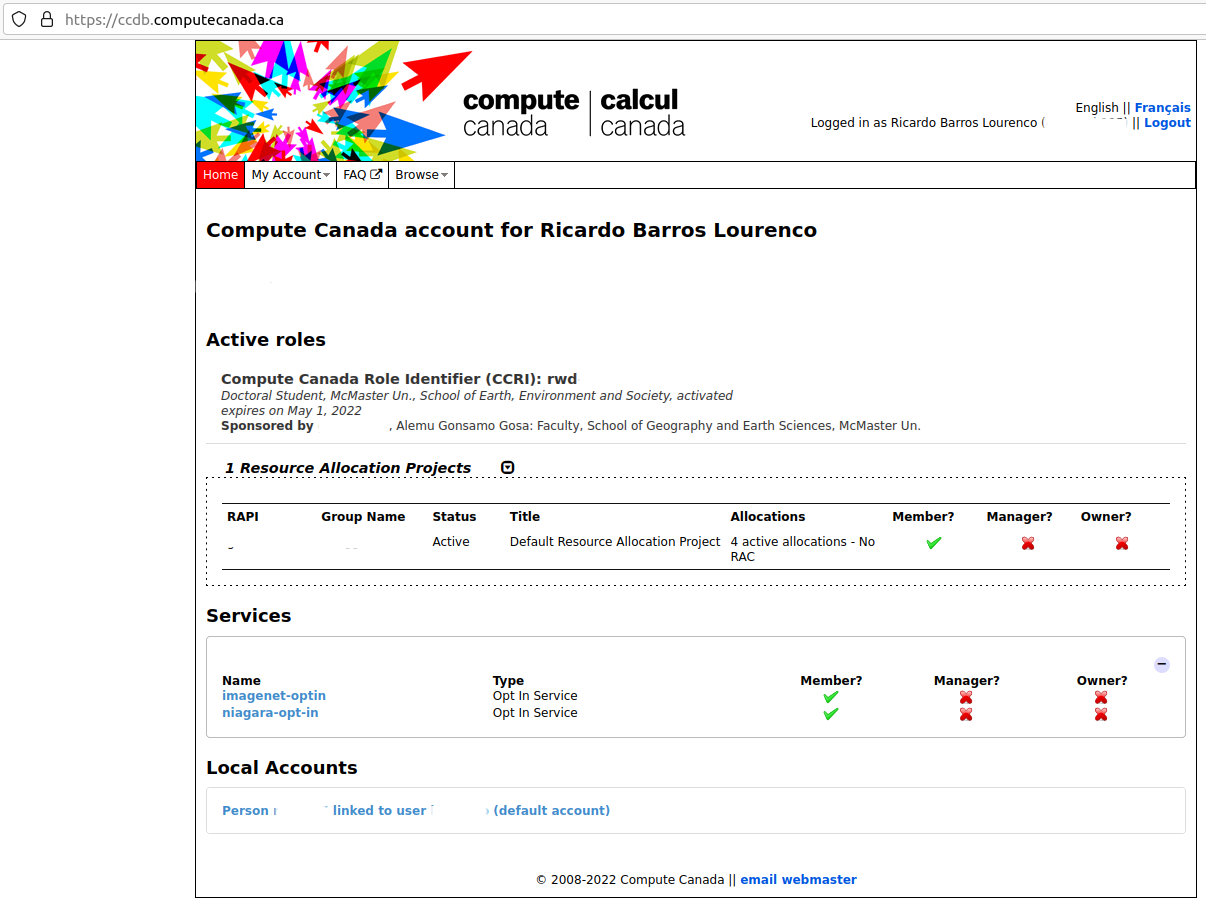
\includegraphics[width=1\linewidth]{images/cc_accnt_01} \caption{Landing page of your Compute Canada account}\label{fig:figure1}
  \end{figure}
\item
  Enter in the \emph{My Account} tab, then click \emph{Manage SSH Keys}:

  \begin{figure}
  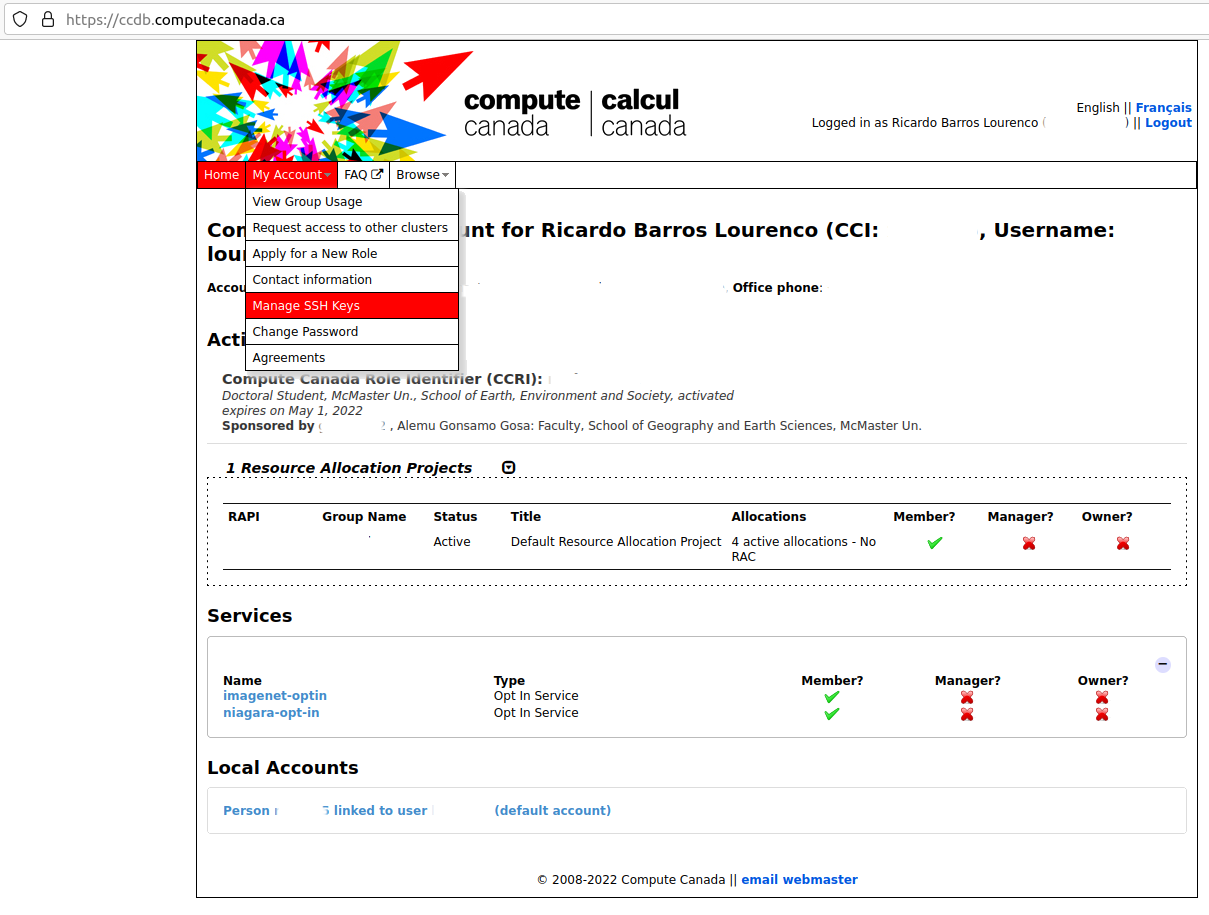
\includegraphics[width=1\linewidth]{images/cc_accnt_02} \caption{Manage SSH Keys menu}\label{fig:figure2}
  \end{figure}
\item
  Then you should have the SSH Key management options:

  \begin{figure}
  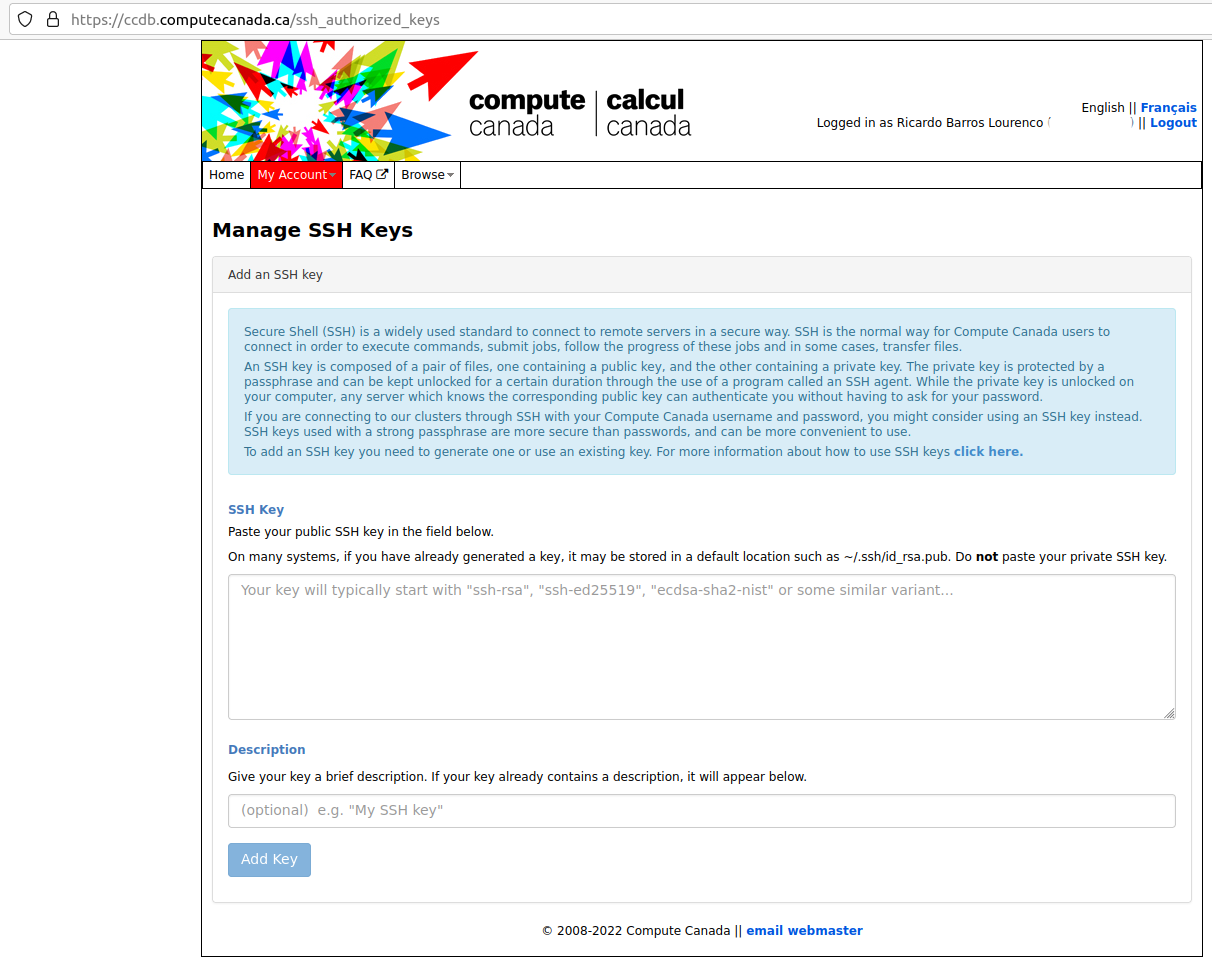
\includegraphics[width=1\linewidth]{images/cc_accnt_03} \caption{SSH Key Management options}\label{fig:figure3}
  \end{figure}
\item
  Now insert the content of your SSH \emph{public key} in the first field.
  To do so, you need to open your \emph{.pub} file with a simple text editor (ex.: Notepad on Windows, TextEdit on MacOS, Gedit/Vi/Emacs on Linux - Do not open with text processing software, as MS Word!) select all content and copy-paste into the first text box.
\item
  Then you should assign a \emph{Description} to such key. I recommend that you use different keys for every system you use to connect to Compute Canada Systems, and this field should reflect each of these systems. For example, a description as such ``\emph{Desktop Machine at the Laboratory}'', or ``\emph{Personal Laptop}'' would be enough to identify where these keys lie (especially important if you get hacked and someone steals your key).
\item
  Then hit \emph{Add Key}. This operation will put your public key on every machine of Compute Canada, and may take up to 30 minutes to be online.
\end{itemize}

\hypertarget{accessing-a-compute-canada-login-node}{%
\section{\texorpdfstring{Accessing a Compute Canada \emph{login node}}{Accessing a Compute Canada login node}}\label{accessing-a-compute-canada-login-node}}

Once your public key is loaded and synchronized in all machines, you may login a compute node using a terminal (On Windows, you need to use PowerShell; on MacOS, Terminal; and on Linux, your preferred Shell, such as Bash):

\begin{Shaded}
\begin{Highlighting}[]
\FunctionTok{ssh} \AttributeTok{{-}i}\NormalTok{ ./computecanada{-}key your{-}compute{-}canada{-}username@MMMMMM.computecanada.ca}
\end{Highlighting}
\end{Shaded}

The command opens a SSH terminal session with the following parameters:

\begin{itemize}
\tightlist
\item
  \emph{-i} : The path and the name of your \emph{Private Key};
\item
  \emph{your-compute-canada-username} : The username you have set for your Compute Canada account, when registering with them for an account;
\item
  \emph{MMMMMM} : One of the Compute Canada clusters (for example, Cedar, Graham, or Beluga)
\end{itemize}

\emph{Note}: We will provide a more extensive list of computing environments later, but for now you may want to refer to \href{http://bit.ly/introhpc}{this presentation}.

\hypertarget{running-batch-jobs}{%
\section{Running batch jobs}\label{running-batch-jobs}}

If you want to run a R-language batch job, please take a look on the
\href{https://github.com/ricardobarroslourenco/CCrecipes}{CCrecipes repository}.

More specifically at the \texttt{slurm/R/r\_batch\_standalone.sh} file, we have:

\begin{Shaded}
\begin{Highlighting}[]
\CommentTok{\#!/bin/bash}

\CommentTok{\#\#\# Sets shell for parallel program (no distribution {-} no MPI)}
\CommentTok{\#\#\# Inspired by the current documentation available on CC Wiki.}

\CommentTok{\#SBATCH {-}{-}account=def{-}someacct             \# replace this with your PI account}
\CommentTok{\#SBATCH {-}{-}nodes=1                          \# number of node MUST be 1}
\CommentTok{\#SBATCH {-}{-}cpus{-}per{-}task=4                  \# number of processes}
\CommentTok{\#SBATCH {-}{-}mem{-}per{-}cpu=2048M                \# memory; default unit is megabytes}
\CommentTok{\#SBATCH {-}{-}time=0{-}00:15                     \# time (DD{-}HH:MM)}
\CommentTok{\#SBATCH {-}{-}mail{-}user=yourname@someplace.com \# Send email updates to you or someone else}
\CommentTok{\#SBATCH {-}{-}mail{-}type=ALL                    \# send an email in all cases (job started, job ended, job aborted)}

\CommentTok{\#\#\# Load library modules}
\ExtensionTok{module}\NormalTok{ load gcc/9.3.0 r/4.0.2}

\CommentTok{\#\#\# Load r{-}packages (builds locally) {-} comment, if unecessary to install new libraries}
\CommentTok{\#R install\_script.R}

\CommentTok{\#\#\# Export locally installed packages}
\CommentTok{\# }\AlertTok{TODO}\CommentTok{: check if this path holds}
\BuiltInTok{export} \VariableTok{R\_LIBS}\OperatorTok{=}\NormalTok{\textasciitilde{}/local/R\_libs/}

\CommentTok{\#\#\# Run main\_job.R {-} or any batch script necessary}
\ExtensionTok{R}\NormalTok{ CMD BATCH }\AttributeTok{{-}{-}no{-}save} \AttributeTok{{-}{-}no{-}restore}\NormalTok{ \textasciitilde{}/main\_job.R}
\end{Highlighting}
\end{Shaded}

Some requirements:

\begin{itemize}
\tightlist
\item
  The R file \texttt{main\_job.R} needs to be at the root of your user folder.
\item
  Also the script needs to be executable (command runned at the same folder
  as \texttt{r\_batch\_standalone.sh}:
\end{itemize}

\begin{Shaded}
\begin{Highlighting}[]
\FunctionTok{chmod}\NormalTok{ +x r\_batch\_standalone.sh}
\end{Highlighting}
\end{Shaded}

\begin{itemize}
\tightlist
\item
  Finally, you can submit this batch job as:
\end{itemize}

\begin{Shaded}
\begin{Highlighting}[]
\ExtensionTok{sbatch}\NormalTok{ r\_batch\_standalone.sh}
\end{Highlighting}
\end{Shaded}

Once submitted, you should receive a job number at the console. Once its status
change at the scheduler (job started, job ended, job aborted), you should receive
an e-mail.

If getting into running issues, take a look on the errors by inspecting the
output files which will be saved at the same folder you submitted the job and
have the name \texttt{slurm-xxxxxx.out} in which \texttt{xxxxxx} is the job number.

\hypertarget{bash}{%
\chapter{BASH}\label{bash}}

On this section we will write some hints on the Bourne Again Shell (BASH), a command interpreter used in several *nix systems, such as Linux, Unix, MacOS and recently incorporated into Windows through PowerShell. This will be more of a collection of hints, and not substituting a full knowledge of BASH and the Operating System in which is running.

\hypertarget{screen}{%
\section{Screen}\label{screen}}

Screen is a tool you can use to keep a ssh session run through BASH alive. Why it is useful(?):

\begin{enumerate}
\def\labelenumi{\arabic{enumi}.}
\tightlist
\item
  When you have unreliable internet connections connections (ex.: Wifi, cellphone);
\item
  Power outages;
\item
  Your local machine freezes, or have any other issue, and your connection is killed;
\item
  Any random reason that blocks your local terminal to access the remote ssh session.
\end{enumerate}

\hypertarget{how-to-use-it}{%
\subsection{How to use it}\label{how-to-use-it}}

Some useful description is available in \href{https://web.archive.org/web/20230606181644/https://www.networkworld.com/article/3441777/how-the-linux-screen-tool-can-save-your-tasks-and-your-sanity-if-ssh-is-interrupted.html}{this website}, and on the app documentation. But you can proceed as follows:

\hypertarget{creating-a-session}{%
\subsection{Creating a session}\label{creating-a-session}}

You create a new session, named \emph{session\_01} as:

\begin{Shaded}
\begin{Highlighting}[]
\ExtensionTok{screen} \AttributeTok{{-}S}\NormalTok{ session\_01}
\end{Highlighting}
\end{Shaded}

\hypertarget{see-all-available-sessions}{%
\subsection{See all available sessions}\label{see-all-available-sessions}}

\begin{Shaded}
\begin{Highlighting}[]
\ExtensionTok{screen} \AttributeTok{{-}ls}
\end{Highlighting}
\end{Shaded}

You probably will see something like this:

\begin{verbatim}
There are screens on:
        6617.session_00      (09/26/2019 04:35:30 PM)    (Detached)
        1946.session_01         (09/26/2019 02:51:50 PM)    (Detached)
2 Sockets in /run/screen/S-shs
\end{verbatim}

\hypertarget{reattach-to-a-previously-established-session}{%
\subsection{Reattach to a previously established session}\label{reattach-to-a-previously-established-session}}

Let's say you want to attach to \emph{session\_00}:

\begin{Shaded}
\begin{Highlighting}[]
\ExtensionTok{screen} \AttributeTok{{-}r}\NormalTok{ session\_00}
\end{Highlighting}
\end{Shaded}

\hypertarget{finishing-a-session}{%
\subsection{Finishing a session}\label{finishing-a-session}}

Let's say you want to finish \emph{session\_01}. You first enter in another session, and:

\begin{Shaded}
\begin{Highlighting}[]
\ExtensionTok{screen} \AttributeTok{{-}XS}\NormalTok{ 1946 quit}
\end{Highlighting}
\end{Shaded}

If the session you are aiming to finish is the last one, then:

\begin{itemize}
\tightlist
\item
  \textbf{ctrl + A};
\item
  \textbf{k};
\item
  and \textbf{y}.
\end{itemize}

\hypertarget{watch}{%
\section{Watch}\label{watch}}

Watch is a program that runs commands using a clock. In our case, watch is kind
of useful when needing to monitor an application shell output. Common cases in HPC
are when you need to see updates in \texttt{nvidia-smi} or slurm \texttt{squeue} command.

The base syntax is:

\begin{Shaded}
\begin{Highlighting}[]
\ExtensionTok{watch} \AttributeTok{{-}n}\NormalTok{ XX command}
\end{Highlighting}
\end{Shaded}

In which:

\begin{itemize}
\tightlist
\item
  \textbf{XX} is the refresh rate in seconds;
\item
  \textbf{command} is the bash command you want to refresh the output
\end{itemize}

\hypertarget{slurm-queue-example}{%
\subsection{Slurm queue example}\label{slurm-queue-example}}

The base syntax is:

\begin{Shaded}
\begin{Highlighting}[]
\ExtensionTok{watch} \AttributeTok{{-}n}\NormalTok{ 5 squeue }\AttributeTok{{-}u}\NormalTok{ username}
\end{Highlighting}
\end{Shaded}

In which:

\begin{itemize}
\tightlist
\item
  \textbf{username} is the username in the slurm cluster;
\end{itemize}

\hypertarget{nvidia-card-output}{%
\subsection{NVIDIA card output}\label{nvidia-card-output}}

The base syntax is:

\begin{Shaded}
\begin{Highlighting}[]
\ExtensionTok{watch} \AttributeTok{{-}n}\NormalTok{ 5 nvidia{-}smi}
\end{Highlighting}
\end{Shaded}

It refreshes every 5 seconds the running info from the NVIDIA card in the node (this will fail on CPU-only nodes)

\hypertarget{rstudio-in-alliance-canada}{%
\chapter{RStudio in Alliance Canada}\label{rstudio-in-alliance-canada}}

\emph{Note 1}: This refers to an experimental usage of RStudio for HPC. This approach
has no official support from the Alliance, and the responsability is solely to
the user. An official R environment is provided, with support, by the Alliance at
\href{https://docs.alliancecan.ca/wiki/Technical_documentation}{this website}.

\emph{Note 2}: This approach is aimed to single node processes. If you want to
explore (or need) distributed processing, we recommend to use the supported
version, and speak with user groups and the Alliance support to help designing routines.

\hypertarget{introduction-1}{%
\section{Introduction}\label{introduction-1}}

In this approach, we use a prestablished \href{https://rocker-project.org/}{RockeR},
docker container from which we expand to our user needs. Binary versions of the
container are available at \href{https://hub.docker.com/repository/docker/ricardobarroslourenco/rstudio_container/general}{Docker Hub}, with the releases and their code available on \href{https://github.com/MacRemoteSensing/rstudio_container/releases}{GitHub}.

\hypertarget{running-an-apptainer-hpc-container-as-an-interactive-session}{%
\section{Running an Apptainer HPC Container as an interactive session}\label{running-an-apptainer-hpc-container-as-an-interactive-session}}

Prior to be able to run RStudio, you need to have a suitable container already built
as a Singularity container, or build by yourself.

\emph{From the cluster login node} you can build it with the following steps (it is assumed that you are using \href{https://en.wikipedia.org/wiki/Bash_(Unix_shell)}{bash} as a regular user - no sudo needed):

\textbf{1. Load Apptainer}:

\begin{Shaded}
\begin{Highlighting}[]
\ExtensionTok{module}\NormalTok{ load apptainer}
\end{Highlighting}
\end{Shaded}

Pick up the most recent version of it (please note that Docker Hub may have
different tags, with versioning for each), and accept.

\textbf{2. Then run the build} (run this command at your \emph{home}, \emph{project} or \emph{scratch} folder):

\begin{Shaded}
\begin{Highlighting}[]
\ExtensionTok{apptainer}\NormalTok{ build rstudio\_container\_v1\_0.sif docker://ricardobarroslourenco/rstudio\_container:v1\_0}
\end{Highlighting}
\end{Shaded}

You should have, at the end, a file named \emph{rstudio\_container\_v1\_0.sif} in the
directory you ran the command. This is your Apptainer container.

\textbf{3. Create transient folders and files to be able to run your container} (these should be hosted at the same location as your container). Creating directories:

\begin{Shaded}
\begin{Highlighting}[]
\FunctionTok{mkdir} \AttributeTok{{-}p}\NormalTok{ run var{-}lib{-}rstudio{-}server .rstudio}
\end{Highlighting}
\end{Shaded}

Then the sqlite configuration file:

\begin{Shaded}
\begin{Highlighting}[]
\BuiltInTok{printf} \StringTok{\textquotesingle{}provider=sqlite\textbackslash{}ndirectory=/var/lib/rstudio{-}server\textbackslash{}n\textquotesingle{}} \OperatorTok{\textgreater{}}\NormalTok{ database.conf}
\end{Highlighting}
\end{Shaded}

\textbf{4. Starting an Interactive Job on the Supercomputer}

\begin{Shaded}
\begin{Highlighting}[]
\ExtensionTok{salloc} \AttributeTok{{-}{-}time}\OperatorTok{=}\NormalTok{0:30:0 }\AttributeTok{{-}{-}account}\OperatorTok{=}\NormalTok{rrg{-}ggalex }\AttributeTok{{-}{-}cpus{-}per{-}task}\OperatorTok{=}\NormalTok{8 }\AttributeTok{{-}{-}mem}\OperatorTok{=}\NormalTok{0 }\AttributeTok{{-}{-}mail{-}user}\OperatorTok{=}\NormalTok{macid@mcmaster.ca }\AttributeTok{{-}{-}mail{-}type}\OperatorTok{=}\NormalTok{ALL}
\end{Highlighting}
\end{Shaded}

The setup of the flags is defined as this (more details available at the Alliance Documentation, as well as on the Slurm manual):

\begin{itemize}
\tightlist
\item
  \emph{time}: time of the interactive session in HH:MM:SS;
\item
  \emph{account}: PI account at the Alliance Can project;
\item
  \emph{cpus-per-task}: Amount of cpus in this interactive session. Capped to the limit of the node;
\item
  \emph{mem}: amount of RAM you want to allocate (zero means all memory of the node);
\item
  \emph{mail-user}: e-mail address to send updates on the job allocation;
\item
  \emph{mail-type}: verbosity of the e-mail.
\end{itemize}

After running this, you probably will see your bash change to something like (in the Graham cluster):

\begin{Shaded}
\begin{Highlighting}[]
\KeywordTok{(}\ExtensionTok{base}\KeywordTok{)} \ExtensionTok{[lourenco@gra{-}login1}\NormalTok{ scratch]$ salloc }\AttributeTok{{-}{-}time}\OperatorTok{=}\NormalTok{0:30:0 }\AttributeTok{{-}{-}account}\OperatorTok{=}\NormalTok{rrg{-}ggalex }\AttributeTok{{-}{-}cpus{-}per{-}task}\OperatorTok{=}\NormalTok{8 }\AttributeTok{{-}{-}mem}\OperatorTok{=}\NormalTok{0 }\AttributeTok{{-}{-}mail{-}user}\OperatorTok{=}\NormalTok{barroslr@mcmaster.ca }\AttributeTok{{-}{-}mail{-}type}\OperatorTok{=}\NormalTok{ALL}
\ExtensionTok{salloc:}\NormalTok{ Pending job allocation 6806097}
\ExtensionTok{salloc:}\NormalTok{ job 6806097 queued and waiting for resources}
\ExtensionTok{salloc:}\NormalTok{ job 6806097 has been allocated resources}
\ExtensionTok{salloc:}\NormalTok{ Granted job allocation 6806097}
\ExtensionTok{salloc:}\NormalTok{ Waiting for resource configuration}
\ExtensionTok{salloc:}\NormalTok{ Nodes gra189 are ready for job}
\KeywordTok{(}\ExtensionTok{base}\KeywordTok{)} \ExtensionTok{[lourenco@gra189}\NormalTok{ scratch]$}
\end{Highlighting}
\end{Shaded}

Please note that \textbf{gra189} in this case is your machine name. You need to remember it later to use it in your ssh tunnel.

\textbf{5. Start the container in the newly allocated working node}

\begin{Shaded}
\begin{Highlighting}[]
\ExtensionTok{apptainer}\NormalTok{ exec }\AttributeTok{{-}{-}bind}\NormalTok{ run:/run,var{-}lib{-}rstudio{-}server:/var/lib/rstudio{-}server,database.conf:/etc/rstudio/database.conf,.rstudio:/home/rstudio/.rstudio/ rstudio\_container\_v1\_0.sif /usr/lib/rstudio{-}server/bin/rserver }\AttributeTok{{-}{-}auth{-}none}\OperatorTok{=}\NormalTok{1 }\AttributeTok{{-}{-}auth{-}pam{-}helper{-}path}\OperatorTok{=}\NormalTok{pam{-}helper }\AttributeTok{{-}{-}server{-}user}\OperatorTok{=}\VariableTok{$(}\FunctionTok{whoami}\VariableTok{)} \AttributeTok{{-}{-}www{-}port}\OperatorTok{=}\NormalTok{8787}
\end{Highlighting}
\end{Shaded}

This will launch an rstudio server as a singularity service. If you need, bash is
available as a terminal tab in that RStudio. To access the instance, you need
to do a ssh tunnel, to forward the cluster port in the working node, to your machine. For that, \textbf{you must to create a new, separate, ssh connection, and keep it open} (without
running any job on it). You can do as this (similar to what we described in the ssh section of CCPrimer, with a twist):

\begin{Shaded}
\begin{Highlighting}[]
\FunctionTok{ssh} \AttributeTok{{-}i}\NormalTok{ \textasciitilde{}/computecanada/computecanada{-}key }\AttributeTok{{-}L}\NormalTok{ 9102:graXXX:8787 username@graham.computecanada.ca}
\end{Highlighting}
\end{Shaded}

Some details:

\begin{itemize}
\tightlist
\item
  \emph{-i \textasciitilde/computecanada/computecanada-key}: the \emph{-i} flag calls your ssh key file;
\item
  \emph{-L 9102:graXXX:8787}: the \emph{ssh tunnel} in fact. It forwards node port 8787 to your localhost at port 9102. Note that \textbf{you must replace graXXX with the node name of the machine assigned to you} after running \emph{salloc};
\item
  \emph{\href{mailto:username@graham.computecanada.ca}{\nolinkurl{username@graham.computecanada.ca}}}: your username, followed by the cluster url. Note that our lab research allocation is available in Graham for now.
\end{itemize}

After this, you should be able to access the rstudio server by using this url
in your browser:

\begin{Shaded}
\begin{Highlighting}[]
\ExtensionTok{localhost:9102}
\end{Highlighting}
\end{Shaded}

\hypertarget{finishing-your-running-session}{%
\section{Finishing your Running session}\label{finishing-your-running-session}}

Do not forget saving your work in partitions that enable saving (ex.: \texttt{/home}, \texttt{/project}, \texttt{/scratch}), because \textbf{if you save in a folder within the container, it will not be saved}, after your session ends. Remember that \texttt{/scratch} is meant for temporary save, being automatically wiped by the cluster systems after 30 days.

Once saved, you can simply end your running sessions by either using \texttt{Ctrl\ +\ C} in the apptainer run session, and then calling \texttt{exit} on bash up to ending the \texttt{salloc} session, and another time, to relinquish the ssh session (remember to do this both in the bash session that runs the jobs, as well in the ssh tunnel). At the end you will only see the bash of your local machine. It is important to do this procedure, because otherwise it may be possible that the machine is still running, and consument the group Alliance Canada credits. Once you finish the slurm \texttt{salloc} session you will receive an e-mail (as you got one when the session started), telling that the session has finished (or relinquished, if your runnign time expired).

\hypertarget{jupyterhub-in-alliance-canada}{%
\chapter{JupyterHub in Alliance Canada}\label{jupyterhub-in-alliance-canada}}

\emph{Note 1}: This refers to an experimental usage of Python for HPC. This approach
has no official support from the Alliance, and the responsability is solely to
the user. An official Python environment is provided, with support, by the Alliance at
\href{https://docs.alliancecan.ca/wiki/Python}{this website}.

\emph{Note 2}: This approach is aimed to single node processes. We will address over time cases with multi-node trainings, but this is still under development (usage of the SOSA Stack - \href{https://youtu.be/2SbpEiOM5JE}{video}, \href{https://zenodo.org/record/7857369}{slides}). However, multi-node multi-gpu Deep Learning models can be already be trained with Horovod in Alliance machines (\href{https://docs.alliancecan.ca/wiki/TensorFlow/en\#Horovod}{link}).

\hypertarget{introduction-2}{%
\section{Introduction}\label{introduction-2}}

In this approach, we use an adaptation of a Docker container maintained by the \href{https://pangeo.io}{Pangeo Community} to install a custom setup of packages from the \href{https://conda-forge.org}{Conda-Forge} project. Containers are available at \href{https://hub.docker.com/repository/docker/ricardobarroslourenco/ts_rs/general}{Docker Hub}, with the releases and their code available on \href{https://github.com/ricardobarroslourenco/rs_images}{GitHub}.

\hypertarget{running-an-apptainer-hpc-container-as-an-interactive-session-1}{%
\section{Running an Apptainer HPC Container as an interactive session}\label{running-an-apptainer-hpc-container-as-an-interactive-session-1}}

Prior to be able to run JupyterLab, you need to have a suitable container already built
as a Singularity container, or build by yourself.

\emph{From the cluster login node} you can build it with the following steps (it is assumed that you are using \href{https://en.wikipedia.org/wiki/Bash_(Unix_shell)}{bash} as a regular user - no sudo needed):

\textbf{1. Load Apptainer}:

\begin{Shaded}
\begin{Highlighting}[]
\ExtensionTok{module}\NormalTok{ load apptainer}
\end{Highlighting}
\end{Shaded}

Pick up the most recent version of it (note that there may be different tags, each one with its own versioning), and accept.

\textbf{2. Then run the build} (run this command at your \emph{home}, \emph{project} or \emph{scratch} folder):

\begin{Shaded}
\begin{Highlighting}[]
\ExtensionTok{apptainer}\NormalTok{ build ts\_rs\_v0\_5.sif docker://ricardobarroslourenco/ts\_rs:v0.5}
\end{Highlighting}
\end{Shaded}

You should have, at the end, a file named \emph{ts\_rs\_v0\_5.sif} in the
directory you ran the command. This is your Apptainer container.

\textbf{3. Starting an Interactive Job on the Supercomputer}
With CPU support in Graham

\begin{Shaded}
\begin{Highlighting}[]
\ExtensionTok{salloc} \AttributeTok{{-}{-}time}\OperatorTok{=}\NormalTok{24:00:0 }\AttributeTok{{-}{-}account}\OperatorTok{=}\NormalTok{rrg{-}ggalex }\AttributeTok{{-}{-}cpus{-}per{-}task}\OperatorTok{=}\NormalTok{44 }\AttributeTok{{-}{-}mem}\OperatorTok{=}\NormalTok{0 }\AttributeTok{{-}{-}mail{-}user}\OperatorTok{=}\NormalTok{macid@mcmaster.ca }\AttributeTok{{-}{-}mail{-}type}\OperatorTok{=}\NormalTok{ALL}
\end{Highlighting}
\end{Shaded}

With GPU (P100) support in Graham

\begin{Shaded}
\begin{Highlighting}[]
\ExtensionTok{salloc} \AttributeTok{{-}{-}time}\OperatorTok{=}\NormalTok{24:00:0 }\AttributeTok{{-}{-}nodes}\OperatorTok{=}\NormalTok{1 }\AttributeTok{{-}{-}gpus{-}per{-}node}\OperatorTok{=}\NormalTok{p100:2 }\AttributeTok{{-}{-}ntasks{-}per{-}node}\OperatorTok{=}\NormalTok{32 }\AttributeTok{{-}{-}mem}\OperatorTok{=}\NormalTok{0 }\AttributeTok{{-}{-}account}\OperatorTok{=}\NormalTok{rrg{-}ggalex }\AttributeTok{{-}{-}mail{-}user}\OperatorTok{=}\NormalTok{macid@mcmaster.ca }\AttributeTok{{-}{-}mail{-}type}\OperatorTok{=}\NormalTok{ALL}
\end{Highlighting}
\end{Shaded}

The setup of the flags is defined as this (more details available at the Alliance Documentation, as well as on the Slurm manual):

\begin{itemize}
\tightlist
\item
  \emph{time}: time of the interactive session in HH:MM:SS;
\item
  \emph{account}: PI account at the Alliance Can project;
\item
  \emph{cpus-per-task}: Amount of cpus in this interactive session. Capped to the limit of the node;
\item
  \emph{mem}: amount of RAM you want to allocate (zero means all memory of the node);
\item
  \emph{mail-user}: e-mail address to send updates on the job allocation;
\item
  \emph{mail-type}: verbosity of the e-mail.
\end{itemize}

After running this, you probably will see your bash change to something like (in the Graham cluster):

\begin{Shaded}
\begin{Highlighting}[]
\KeywordTok{(}\ExtensionTok{base}\KeywordTok{)} \ExtensionTok{[lourenco@gra{-}login1}\NormalTok{ scratch]$ salloc }\AttributeTok{{-}{-}time}\OperatorTok{=}\NormalTok{0:30:0 }\AttributeTok{{-}{-}account}\OperatorTok{=}\NormalTok{rrg{-}ggalex }\AttributeTok{{-}{-}cpus{-}per{-}task}\OperatorTok{=}\NormalTok{8 }\AttributeTok{{-}{-}mem}\OperatorTok{=}\NormalTok{0 }\AttributeTok{{-}{-}mail{-}user}\OperatorTok{=}\NormalTok{barroslr@mcmaster.ca }\AttributeTok{{-}{-}mail{-}type}\OperatorTok{=}\NormalTok{ALL}
\ExtensionTok{salloc:}\NormalTok{ Pending job allocation 6806097}
\ExtensionTok{salloc:}\NormalTok{ job 6806097 queued and waiting for resources}
\ExtensionTok{salloc:}\NormalTok{ job 6806097 has been allocated resources}
\ExtensionTok{salloc:}\NormalTok{ Granted job allocation 6806097}
\ExtensionTok{salloc:}\NormalTok{ Waiting for resource configuration}
\ExtensionTok{salloc:}\NormalTok{ Nodes gra189 are ready for job}
\KeywordTok{(}\ExtensionTok{base}\KeywordTok{)} \ExtensionTok{[lourenco@gra189}\NormalTok{ scratch]$}
\end{Highlighting}
\end{Shaded}

Please note that \textbf{gra189} in this case is your machine name. You need to remember it later to use it in your ssh tunnel.

\textbf{4. Start the container in the newly allocated working node}

\begin{Shaded}
\begin{Highlighting}[]
\ExtensionTok{apptainer}\NormalTok{ shell }\AttributeTok{{-}{-}nv} \AttributeTok{{-}B}\NormalTok{ /home }\AttributeTok{{-}B}\NormalTok{ /project }\AttributeTok{{-}B}\NormalTok{ /scratch ts\_rs\_v0\_5.sif}
\end{Highlighting}
\end{Shaded}

Another option, which mounts all system folders in a single \emph{host\_folders} folder can be assigned as this:

\begin{Shaded}
\begin{Highlighting}[]
\ExtensionTok{apptainer}\NormalTok{ shell }\AttributeTok{{-}{-}nv} \AttributeTok{{-}B}\NormalTok{ \textasciitilde{}/.:/host\_folders/home,/home/lourenco/projects/rrg{-}ggalex/lourenco:/host\_folders/projects\_ricardo,/home/lourenco/scratch:/host\_folders/scratch ts\_rs\_v0\_5.sif}
\end{Highlighting}
\end{Shaded}

\textbf{5. Launching JupyterLab}

The container is now started, and you need now to start JupyterLab. First, load the conda environment on the container:

\begin{Shaded}
\begin{Highlighting}[]
\BuiltInTok{source}\NormalTok{ activate base}
\end{Highlighting}
\end{Shaded}

Note that startting Jupyter on the console will limit the scope of folders that Jupyter can see. I recommend to mount that on the root of the container filesystem. To guarantee that, let's got to the base:

\begin{Shaded}
\begin{Highlighting}[]
\BuiltInTok{cd}\NormalTok{ /}
\end{Highlighting}
\end{Shaded}

Then now start a JupyterLab session (this is a session that is headless):

\begin{Shaded}
\begin{Highlighting}[]
\ExtensionTok{jupyter{-}lab} \AttributeTok{{-}{-}no{-}browser} \AttributeTok{{-}{-}ip} \VariableTok{$(}\FunctionTok{hostname} \AttributeTok{{-}f}\VariableTok{)}
\end{Highlighting}
\end{Shaded}

This will launch a JupyterLab server as a singularity service. If you need, bash is
available as a terminal tab in that JupyterLab. You should see something like this:

\begin{Shaded}
\begin{Highlighting}[]
\ExtensionTok{Apptainer}\OperatorTok{\textgreater{}}\NormalTok{ jupyter{-}lab }\AttributeTok{{-}{-}no{-}browser} \AttributeTok{{-}{-}ip} \VariableTok{$(}\FunctionTok{hostname} \AttributeTok{{-}f}\VariableTok{)}
\ExtensionTok{[I}\NormalTok{ 2023{-}06{-}07 11:36:57.713 ServerApp] Package jupyterlab took 0.0000s to import}
\ExtensionTok{[I}\NormalTok{ 2023{-}06{-}07 11:36:59.595 ServerApp] Package dask\_labextension took 1.8814s to import}
\ExtensionTok{[W}\NormalTok{ 2023{-}06{-}07 11:36:59.595 ServerApp] A }\KeywordTok{\textasciigrave{}}\ExtensionTok{\_jupyter\_server\_extension\_points}\KeywordTok{\textasciigrave{}}\NormalTok{ function was not found in dask\_labextension. Instead, a }\KeywordTok{\textasciigrave{}}\ExtensionTok{\_jupyter\_server\_extension\_paths}\KeywordTok{\textasciigrave{}}\NormalTok{ function was found and will be used for now. This function name will be deprecated in future releases of Jupyter Server.}
\ExtensionTok{[I}\NormalTok{ 2023{-}06{-}07 11:36:59.624 ServerApp] Package jupyter\_lsp took 0.0291s to import}
\ExtensionTok{[W}\NormalTok{ 2023{-}06{-}07 11:36:59.624 ServerApp] A }\KeywordTok{\textasciigrave{}}\ExtensionTok{\_jupyter\_server\_extension\_points}\KeywordTok{\textasciigrave{}}\NormalTok{ function was not found in jupyter\_lsp. Instead, a }\KeywordTok{\textasciigrave{}}\ExtensionTok{\_jupyter\_server\_extension\_paths}\KeywordTok{\textasciigrave{}}\NormalTok{ function was found and will be used for now. This function name will be deprecated in future releases of Jupyter Server.}
\ExtensionTok{[I}\NormalTok{ 2023{-}06{-}07 11:36:59.625 ServerApp] Package jupyter\_server\_proxy took 0.0000s to import}
\ExtensionTok{[I}\NormalTok{ 2023{-}06{-}07 11:36:59.644 ServerApp] Package jupyter\_server\_terminals took 0.0188s to import}
\ExtensionTok{[I}\NormalTok{ 2023{-}06{-}07 11:36:59.644 ServerApp] Package notebook\_shim took 0.0000s to import}
\ExtensionTok{[W}\NormalTok{ 2023{-}06{-}07 11:36:59.644 ServerApp] A }\KeywordTok{\textasciigrave{}}\ExtensionTok{\_jupyter\_server\_extension\_points}\KeywordTok{\textasciigrave{}}\NormalTok{ function was not found in notebook\_shim. Instead, a }\KeywordTok{\textasciigrave{}}\ExtensionTok{\_jupyter\_server\_extension\_paths}\KeywordTok{\textasciigrave{}}\NormalTok{ function was found and will be used for now. This function name will be deprecated in future releases of Jupyter Server.}
\ExtensionTok{[I}\NormalTok{ 2023{-}06{-}07 11:37:01.808 ServerApp] Package panel.io.jupyter\_server\_extension took 2.1617s to import}
\ExtensionTok{[I}\NormalTok{ 2023{-}06{-}07 11:37:01.808 ServerApp] dask\_labextension }\KeywordTok{|} \ExtensionTok{extension}\NormalTok{ was successfully linked.}
\ExtensionTok{[I}\NormalTok{ 2023{-}06{-}07 11:37:01.808 ServerApp] jupyter\_lsp }\KeywordTok{|} \ExtensionTok{extension}\NormalTok{ was successfully linked.}
\ExtensionTok{[I}\NormalTok{ 2023{-}06{-}07 11:37:01.808 ServerApp] jupyter\_server\_proxy }\KeywordTok{|} \ExtensionTok{extension}\NormalTok{ was successfully linked.}
\ExtensionTok{[I}\NormalTok{ 2023{-}06{-}07 11:37:01.813 ServerApp] jupyter\_server\_terminals }\KeywordTok{|} \ExtensionTok{extension}\NormalTok{ was successfully linked.}
\ExtensionTok{[I}\NormalTok{ 2023{-}06{-}07 11:37:01.818 ServerApp] jupyterlab }\KeywordTok{|} \ExtensionTok{extension}\NormalTok{ was successfully linked.}
\ExtensionTok{[I}\NormalTok{ 2023{-}06{-}07 11:37:02.927 ServerApp] notebook\_shim }\KeywordTok{|} \ExtensionTok{extension}\NormalTok{ was successfully linked.}
\ExtensionTok{[I}\NormalTok{ 2023{-}06{-}07 11:37:02.927 ServerApp] panel.io.jupyter\_server\_extension }\KeywordTok{|} \ExtensionTok{extension}\NormalTok{ was successfully linked.}
\ExtensionTok{[I}\NormalTok{ 2023{-}06{-}07 11:37:02.972 ServerApp] notebook\_shim }\KeywordTok{|} \ExtensionTok{extension}\NormalTok{ was successfully loaded.}
\ExtensionTok{[I}\NormalTok{ 2023{-}06{-}07 11:37:02.973 ServerApp] dask\_labextension }\KeywordTok{|} \ExtensionTok{extension}\NormalTok{ was successfully loaded.}
\ExtensionTok{[I}\NormalTok{ 2023{-}06{-}07 11:37:02.975 ServerApp] jupyter\_lsp }\KeywordTok{|} \ExtensionTok{extension}\NormalTok{ was successfully loaded.}
\ExtensionTok{[I}\NormalTok{ 2023{-}06{-}07 11:37:02.996 ServerApp] jupyter\_server\_proxy }\KeywordTok{|} \ExtensionTok{extension}\NormalTok{ was successfully loaded.}
\ExtensionTok{[I}\NormalTok{ 2023{-}06{-}07 11:37:02.997 ServerApp] jupyter\_server\_terminals }\KeywordTok{|} \ExtensionTok{extension}\NormalTok{ was successfully loaded.}
\ExtensionTok{[I}\NormalTok{ 2023{-}06{-}07 11:37:02.998 LabApp] JupyterLab extension loaded from /opt/conda/lib/python3.11/site{-}packages/jupyterlab}
\ExtensionTok{[I}\NormalTok{ 2023{-}06{-}07 11:37:02.998 LabApp] JupyterLab application directory is /opt/conda/share/jupyter/lab}
\ExtensionTok{[I}\NormalTok{ 2023{-}06{-}07 11:37:02.999 LabApp] Extension Manager is }\StringTok{\textquotesingle{}pypi\textquotesingle{}}\NormalTok{.}
\ExtensionTok{[I}\NormalTok{ 2023{-}06{-}07 11:37:03.001 ServerApp] jupyterlab }\KeywordTok{|} \ExtensionTok{extension}\NormalTok{ was successfully loaded.}
\ExtensionTok{[I}\NormalTok{ 2023{-}06{-}07 11:37:03.001 ServerApp] panel.io.jupyter\_server\_extension }\KeywordTok{|} \ExtensionTok{extension}\NormalTok{ was successfully loaded.}
\ExtensionTok{[I}\NormalTok{ 2023{-}06{-}07 11:37:03.002 ServerApp] Serving notebooks from local directory: /scratch/lourenco}
\ExtensionTok{[I}\NormalTok{ 2023{-}06{-}07 11:37:03.002 ServerApp] Jupyter Server 2.6.0 is running at:}
\ExtensionTok{[I}\NormalTok{ 2023{-}06{-}07 11:37:03.002 ServerApp] http://gra{-}login2.graham.sharcnet:8888/lab}\PreprocessorTok{?}\NormalTok{token=4ccce5d0045ff5768194c8c7f37a7dc80220caaf68324b8b}
\ExtensionTok{[I}\NormalTok{ 2023{-}06{-}07 11:37:03.002 ServerApp]     http://127.0.0.1:8888/lab}\PreprocessorTok{?}\NormalTok{token=4ccce5d0045ff5768194c8c7f37a7dc80220caaf68324b8b}
\ExtensionTok{[I}\NormalTok{ 2023{-}06{-}07 11:37:03.002 ServerApp] Use Control{-}C to stop this server and shut down all kernels }\ErrorTok{(}\ExtensionTok{twice}\NormalTok{ to skip confirmation}\KeywordTok{)}\BuiltInTok{.}
\ExtensionTok{[C}\NormalTok{ 2023{-}06{-}07 11:37:03.028 ServerApp] }
    
    \ExtensionTok{To}\NormalTok{ access the server, open this file in a browser:}
        \ExtensionTok{file:///home/lourenco/.local/share/jupyter/runtime/jpserver{-}11176{-}open.html}
    \ExtensionTok{Or}\NormalTok{ copy and paste one of these URLs:}
        \ExtensionTok{http://gra{-}login2.graham.sharcnet:8888/lab?token=4ccce5d0045ff5768194c8c7f37a7dc80220caaf68324b8b}
        \ExtensionTok{http://127.0.0.1:8888/lab?token=4ccce5d0045ff5768194c8c7f37a7dc80220caaf68324b8b}
\end{Highlighting}
\end{Shaded}

Note that despite several url's are provided to access the JupyterLab server, the server does not know that is running withing a container, in a cluster, therefore such URLs do not immediately work, as you are accessing it through a tunnel. The only one able to access, \textbf{after creating the ssh tunnel on port 8888}, is \texttt{http://127.0.0.1:8888/lab?token=4ccce5d0045ff5768194c8c7f37a7dc80220caaf68324b8b}.

Reinforcing, to access the instance, you need
to do a ssh tunnel, to forward the cluster port in the working node, to your machine. For that, \textbf{you must to create a new, separate, ssh connection, and keep it open} (without
running any job on it). You can do as this (similar to what we described in the ssh section of CCPrimer, with a twist):

\begin{Shaded}
\begin{Highlighting}[]
\FunctionTok{ssh} \AttributeTok{{-}i}\NormalTok{ \textasciitilde{}/computecanada/computecanada{-}key }\AttributeTok{{-}L}\NormalTok{ 8888:graXXX:8888 username@graham.computecanada.ca}
\end{Highlighting}
\end{Shaded}

Some details:

\begin{itemize}
\tightlist
\item
  \emph{-i \textasciitilde/computecanada/computecanada-key}: the \emph{-i} flag calls your ssh key file;
\item
  \emph{-L 8888:graXXX:8888}: the \emph{ssh tunnel} in fact. It forwards node port 8888 to your localhost at port 8888. Note that \textbf{you must replace graXXX with the node name of the machine assigned to you} after running \emph{salloc}. If you use Dask in your jobs, it is available within the 8888, not needing to open aditional ports for the dashboards;
\item
  \emph{\href{mailto:username@graham.computecanada.ca}{\nolinkurl{username@graham.computecanada.ca}}}: your username, followed by the cluster url. Note that our lab research allocation is available in Graham for now.
\end{itemize}

After this, you should be able to access the rstudio server by using this url
in your browser:

\begin{Shaded}
\begin{Highlighting}[]
\ExtensionTok{http://127.0.0.1:8888/lab?token=XXXXXXXXXXXXXXXXXXXXXXX}
\end{Highlighting}
\end{Shaded}

Remember that this is an example, so you need to get the token URL provided by JupyterLab once launching the session.

\hypertarget{finishing-your-running-session-1}{%
\section{Finishing your Running session}\label{finishing-your-running-session-1}}

Do not forget saving your work in partitions that enable saving (ex.: \texttt{/home}, \texttt{/project}, \texttt{/scratch}), because \textbf{if you save in a folder within the container, it will not be saved}, after your session ends. Remember that \texttt{/scratch} is meant for temporary save, being automatically wiped by the cluster systems after 30 days.

Once saved, you can simply end your running sessions by either using \texttt{Ctrl\ +\ C} in the apptainer run session, and then calling \texttt{exit} on bash up to ending the \texttt{salloc} session, and another time, to relinquish the ssh session (remember to do this both in the bash session that runs the jobs, as well in the ssh tunnel). At the end you will only see the bash of your local machine. It is important to do this procedure, because otherwise it may be possible that the machine is still running, and consument the group Alliance Canada credits. Once you finish the slurm \texttt{salloc} session you will receive an e-mail (as you got one when the session started), telling that the session has finished (or relinquished, if your runnign time expired).

\hypertarget{globus}{%
\chapter{Globus}\label{globus}}

Globus is currently a suite of products for Computational Science.
Initially defined as a tool that allowed the establishment of federations,
now it offers a platform that can do, among many features, distributed data
transfers. When referring in this guide to Globus, the author majorly means
Globus Transfer capabilities.

\hypertarget{documentation}{%
\section{Documentation}\label{documentation}}

A full documentation of Globus is provided aat their website: \url{https://docs.globus.org}

Additional information on how to create an account using the Compute Canada credentials can be found here: \url{https://docs.alliancecan.ca/wiki/Globus}

  \bibliography{book.bib,packages.bib}

\end{document}
